% !TeX program = xelatex
% AI for Theological Inquiry — Lecture 1 deck. Build: xelatex lecture01.tex (twice).
% beamer-slides house preamble.
% Copy into a new deck and edit \deckauthor / \deckemail / \deckdate / colors.
% Build: xelatex deck.tex (run twice). See ../SKILL.md for the full house style.
\documentclass[aspectratio=169,11pt]{beamer}

\usetheme{metropolis}
\usepackage{fontspec}
\usepackage{graphicx}
\usepackage{tikz}
\usetikzlibrary{arrows.meta,positioning,shapes.geometric,fit,shadows}
\usepackage{tcolorbox}
\tcbuselibrary{skins,breakable}
\usepackage{fontawesome5}
\usepackage{listings}
\usepackage{booktabs}
\usepackage{array}

% ---------------------------------------------------------------- palette
% Placeholder professional navy/accent palette — swap for the exact ANL/ALCF
% brand hex values if you have the brand guide; do not present these as
% "official" institutional colors.
\definecolor{labnavy}{RGB}{18,42,73}
\definecolor{labink}{RGB}{40,44,52}
\definecolor{accentgold}{RGB}{223,161,54}
\definecolor{accentteal}{RGB}{0,137,123}
\definecolor{accentblue}{RGB}{41,98,168}
\definecolor{lightgray}{RGB}{245,246,248}
\definecolor{midgray}{RGB}{110,118,129}

% Hard rule: background is always white.
\setbeamercolor{background canvas}{bg=white}
\setbeamercolor{palette primary}{bg=labnavy,fg=white}
\setbeamercolor{frametitle}{bg=labnavy,fg=white}
\setbeamercolor{progress bar}{fg=accentteal,bg=lightgray}
\setbeamercolor{normal text}{fg=labink}
\setbeamercolor{alerted text}{fg=accentgold}
\setbeamercolor{footline}{fg=midgray}
\setbeamerfont{footline}{size=\tiny}

% Tighter default itemize indentation (see SKILL.md Gotchas — do NOT pass
% [leftmargin=...] to Beamer's itemize, that slot is for overlay specs).
\setlength{\leftmargini}{14pt}

% ---------------------------------------------------------------- deck metadata
% Fill these in per-deck. Email + date are a hard rule on the title page.
\newcommand{\deckauthor}{Huihuo Zheng}
\newcommand{\deckemail}{huihuo.zheng@wheaton.edu}
\newcommand{\deckinstitute}{Wheaton College}
% \date{...} still needs to be called explicitly in the document, e.g. \date{\today}

% ---------------------------------------------------------------- logo
% Looks for a real logo file first; falls back to a plain text lockup rather
% than fabricating the institutional mark. Put the real file at
% logos/argonne_logo.pdf (or .png) next to the deck, or point this at a
% shared assets/logos/ path.
% Drop a real logo at logos/wheaton_logo.pdf (or .png) to use it; otherwise
% this falls back to a plain text lockup rather than fabricating the mark.
\newcommand{\decklogo}[1][0.16\textwidth]{%
  \IfFileExists{logos/wheaton_logo.pdf}%
    {
\includegraphics[width=#1]{logos/wheaton_logo.pdf}}%
    {\IfFileExists{logos/wheaton_logo.png}%
      {
\includegraphics[width=#1]{logos/wheaton_logo.png}}%
      {\begin{minipage}{#1}\centering
         {\Large\bfseries\textsc{\textcolor{labnavy}{Wheaton}}}\\[1pt]
         {\small\bfseries\textsc{\textcolor{labnavy}{College}}}
       \end{minipage}}}%
}

% Small corner logo on every content slide (title page uses \decklogo directly
% instead, usually larger — see templates/titlepage.tex). Comment out this
% \logo{} line if you don't want the small footer/corner logo repeated.
% Teaching deck: no repeated corner logo (title page carries it once).
% \logo{\IfFileExists{logos/argonne_logo.pdf}%
%   {\includegraphics[height=0.45cm]{logos/argonne_logo.pdf}}%
%   {\IfFileExists{logos/argonne_logo.png}%
%     {\includegraphics[height=0.45cm]{logos/argonne_logo.png}}{}}}

% ---------------------------------------------------------------- shadowed boxes
% House rule: every box gets a shadow. Pick "drop shadow" (crisp) or
% "drop fuzzy shadow" (soft) and use it consistently through one deck.
% IMPORTANT: "enhanced" is required for the shadow to render at all — without
% it tcolorbox silently accepts the "drop shadow"/"drop fuzzy shadow" key and
% draws nothing (no error, no warning). See SKILL.md Gotchas.
\newtcolorbox{featbox}[2]{
  enhanced,
  colback=lightgray, colframe=#1, boxrule=0.6pt, arc=3pt,
  left=6pt, right=6pt, top=4pt, bottom=4pt,
  title=#2, colbacktitle=#1, coltitle=white,
  fonttitle=\bfseries\small, boxsep=1pt,
  drop fuzzy shadow
}

\newtcolorbox{calloutbox}[1][labnavy]{
  enhanced,
  colback=#1!6, colframe=#1, boxrule=0.6pt, arc=3pt,
  left=10pt, right=10pt, top=6pt, bottom=6pt,
  drop fuzzy shadow
}

\lstdefinestyle{shell}{
  basicstyle=\ttfamily\scriptsize\color{labink},
  keywordstyle=\color{accentblue}\bfseries,
  commentstyle=\color{midgray}\itshape,
  stringstyle=\color{accentteal},
  backgroundcolor=\color{lightgray},
  frame=single, framerule=0.4pt, rulecolor=\color{midgray!60},
  breaklines=true, columns=fullflexible,
  xleftmargin=4pt, xrightmargin=4pt, framexleftmargin=4pt
}


% ---- palette aliases for this deck's three pillars ----
\definecolor{cAgent}{RGB}{41,98,168}   % agentic AI  (blue)
\definecolor{cRAG}{RGB}{0,137,123}     % RAG         (teal)
\definecolor{cEval}{RGB}{223,161,54}   % evaluation  (gold)

\title{AI for Theological Inquiry}
\subtitle{Lecture 1 — The course, agentic AI, and your toolkit}
\date{September 2, 2026}

\begin{document}

% beamer-slides house title page.
% Requires preamble.tex to be loaded first (\decklogo, \deckauthor, \deckemail,
% \deckinstitute). Set \title{}/\subtitle{} and \date{} before this frame.
%
% Hard rule: title page always shows author name, email, and date. Email sits
% bottom-left in small type, footnote-style — not in the author block.

\begin{frame}[plain]
  \begin{columns}[c]
    \begin{column}{0.32\textwidth}
      \centering
      \decklogo[0.9\textwidth]
    \end{column}
    \begin{column}{0.66\textwidth}
      {\usebeamerfont{title}\usebeamercolor[fg]{title}\Huge\bfseries \inserttitle\par}
      \ifx\insertsubtitle\@empty\else
        \vspace{4pt}
        {\large\color{midgray}\insertsubtitle\par}
      \fi
      \vspace{18pt}
      {\small
        \deckauthor\\
        \deckinstitute\\
        \insertdate}
    \end{column}
  \end{columns}
  \vfill
  {\footnotesize\color{midgray}\deckemail\par}
\end{frame}


% ---------------------------------------------------------------- course description
\begin{frame}{Course description}
  \begin{center}\footnotesize\color{midgray}
    Originally: \emph{Knowledge-Based AI for Theological Inquiry and Text Analysis}
  \end{center}
  \vspace{4pt}
  \begin{calloutbox}[labnavy]
    \small
    Exploration of the applications of artificial intelligence to \textbf{theological
    texts} and \textbf{multi-perspective question answering}. Topics include
    \textcolor{cRAG}{\textbf{retrieval-augmented generation}},
    \textcolor{cRAG}{\textbf{vector databases}},
    \textcolor{cRAG}{\textbf{knowledge graphs}},
    \textcolor{cAgent}{\textbf{AI agents}}, and
    \textcolor{cEval}{\textbf{evaluation of attribution, faithfulness, and bias}}
    in generated responses.
  \end{calloutbox}
  \vspace{8pt}
  \begin{center}
  \begin{minipage}{0.9\textwidth}\small
    Students participate in a \textbf{collaborative research project}: the design,
    construction, and evaluation of a knowledge-based AI system for
    multi-perspective theological question answering.
  \end{minipage}
  \end{center}
  \vspace{8pt}
  \begin{center}\footnotesize\color{midgray}%
    \faLock\ Limited enrollment $\cdot$ faculty approval required.\end{center}
\end{frame}

% ---------------------------------------------------------------- agenda
\begin{frame}{Today: one lecture, one hands-on setup}
  \begin{columns}[t, totalwidth=\textwidth]
    \begin{column}{0.47\textwidth}
      \begin{featbox}{accentblue}{\faChalkboardTeacher\ Part 1 — Lecture}
        \small
        \begin{itemize}
          \item What this course is
          \item The syllabus \& the 4 phases
          \item The mentored-research structure
          \item A first look at \textbf{agentic AI}
        \end{itemize}
      \end{featbox}
    \end{column}
    \begin{column}{0.06\textwidth}\end{column}
    \begin{column}{0.47\textwidth}
      \begin{featbox}{accentteal}{\faLaptopCode\ Part 2 — Hands-on}
        \small
        \begin{itemize}
          \item Install VS Code
          \item Install a coding agent:\\ \textbf{Claude Code} or \textbf{Codex}
          \item Feel the agent loop yourself
        \end{itemize}
      \end{featbox}
    \end{column}
  \end{columns}
  \vspace{10pt}
  \begin{center}
    \small\color{midgray}Goal: you leave with the plan, the intuition, and a working environment.
  \end{center}
\end{frame}

% ---------------------------------------------------------------- three pillars
\begin{frame}{Three pillars, and they build on each other}
  \begin{columns}[t, totalwidth=\textwidth]
    \begin{column}{0.31\textwidth}
      \begin{featbox}{cAgent}{\faRobot\ Agentic AI}
        \small The system that \textbf{plans}, uses \textbf{tools}, and
        \textbf{acts} over many steps.
      \end{featbox}
    \end{column}
    \begin{column}{0.035\textwidth}\end{column}
    \begin{column}{0.31\textwidth}
      \begin{featbox}{cRAG}{\faDatabase\ RAG}
        \small How it stays \textbf{grounded in real texts} instead of
        inventing them.
      \end{featbox}
    \end{column}
    \begin{column}{0.035\textwidth}\end{column}
    \begin{column}{0.31\textwidth}
      \begin{featbox}{cEval}{\faCheckDouble\ Evaluation}
        \small How you \textbf{know} whether any of it is trustworthy.
      \end{featbox}
    \end{column}
  \end{columns}
  \vspace{14pt}
  \begin{center}
    {\large\bfseries
      \textcolor{cRAG}{Ground it.}\quad
      \textcolor{cAgent}{Make it act.}\quad
      \textcolor{cEval}{Prove it works.}}
  \end{center}
\end{frame}

% ---------------------------------------------------------------- the key line
\begin{frame}{Why evaluation gets equal weight}
  \vspace{6pt}
  \begin{calloutbox}[accentgold]
    \large\faExclamationTriangle\ \textbf{In theology, a fabricated scripture
    reference is a scholarly \emph{and} pastoral failure.}
  \end{calloutbox}
  \vspace{14pt}
  \begin{center}
  \begin{minipage}{0.86\textwidth}
    \small
    A language model is fluent and confident --- and will happily produce a
    plausible, \emph{non-existent} verse. So we do not trust its claims;
    we \textbf{check} them. That is why we spend as much time on evaluation
    as on building.
  \end{minipage}
  \end{center}
\end{frame}

% ---------------------------------------------------------------- syllabus phases
\begin{frame}{14 weeks, four phases, one project through-line}
  \begin{center}
  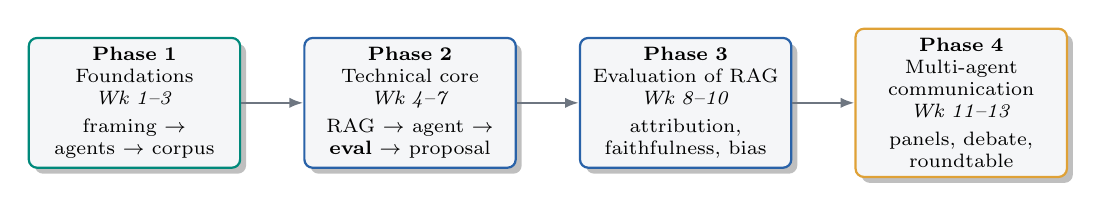
\begin{tikzpicture}[
      font=\scriptsize,
      ph/.style={rectangle, rounded corners=3pt, draw, thick, align=center,
                 text width=2.45cm, minimum height=1.55cm, drop shadow,
                 fill=lightgray},
    ]
    \node[ph, draw=cRAG]   (p1) at (0,0)   {\textbf{Phase 1}\\ Foundations\\ \textit{Wk 1--3}\\[2pt] framing $\to$ agents $\to$ corpus};
    \node[ph, draw=cAgent] (p2) at (3.5,0) {\textbf{Phase 2}\\ Technical core\\ \textit{Wk 4--7}\\[2pt] RAG $\to$ agent $\to$ \textbf{eval} $\to$ proposal};
    \node[ph, draw=accentblue] (p3) at (7,0) {\textbf{Phase 3}\\ Evaluation of RAG\\ \textit{Wk 8--10}\\[2pt] attribution, faithfulness, bias};
    \node[ph, draw=cEval]  (p4) at (10.5,0){\textbf{Phase 4}\\ Multi-agent\\ communication\\ \textit{Wk 11--13}\\[2pt] panels, debate, roundtable};
    \draw[-{Latex[length=5pt]}, midgray, thick] (p1) -- (p2);
    \draw[-{Latex[length=5pt]}, midgray, thick] (p2) -- (p3);
    \draw[-{Latex[length=5pt]}, midgray, thick] (p3) -- (p4);
  \end{tikzpicture}
  \end{center}
  \vspace{8pt}
  \begin{center}
    \begin{tikzpicture}
      \node[rectangle, rounded corners=3pt, draw=labnavy, thick, fill=labnavy!8,
            drop shadow, align=center, text width=4.2cm, font=\scriptsize,
            minimum height=0.9cm]
        {\textbf{\faTrophy\ Week 14 --- Symposium}\\ final paper + presentation};
    \end{tikzpicture}
  \end{center}
  \vspace{4pt}
  \begin{center}\small\color{midgray}Each week: $\sim$40 min concept $\cdot$ $\sim$40 min lab $\cdot$ $\sim$20 min project touchpoint.\end{center}
\end{frame}

% ---------------------------------------------------------------- deliverables
\begin{frame}{How you are graded}
  \vfill
  \begin{center}
    \begin{tabular}{@{}p{5.5cm}r@{}}
      \toprule
      \Large\textbf{Component} & \Large\textbf{Weight}\\
      \midrule
      \Large Participation   & \Large\color{cAgent}\textbf{40\%}\\[4pt]
      \Large Paper           & \Large\color{cRAG}\textbf{30\%}\\[4pt]
      \Large Presentation    & \Large\color{cEval}\textbf{30\%}\\
      \bottomrule
    \end{tabular}
  \end{center}
  \vfill
\end{frame}

% ---------------------------------------------------------------- mentored research
\begin{frame}{What ``mentored research'' means for you}
  \setlength{\leftmargini}{16pt}
  \begin{itemize}\small
    \item \textbf{One original project all term} --- a researchable
      theological question + an agentic method + an \textbf{evaluation plan}.
    \item \textbf{Continuous mentoring} --- weekly 20-min touchpoints, so you
      never drift far before a check-in.
    \item \textbf{Low-code by default} --- you build from provided notebook
      templates; an optional \textbf{light-code (Python)} path exists.
      \emph{No one writes an agent or eval harness from scratch.}
    \item \textbf{One corpus, one agent} --- RAG (Wk 4) grounds the agent
      (Wk 5); evaluation (Wk 6) judges both. Same texts all term.
  \end{itemize}
  \vspace{4pt}
  \begin{center}\small\color{labnavy}\bfseries Ground it. Make it act. Prove it works --- on \emph{your} question.\end{center}
\end{frame}

% ---------------------------------------------------------------- history of AI (arc)
% Recreated in-deck from ATPESC 2026 "History of AI and Agentic AI" (agentic_tools_1)
% + "Five overlapping waves" (intro_to_deep_learning_Zheng). Source .tex not on disk.
\begin{frame}{A short history of AI: from predicting to acting}
  \begin{center}
  \begin{tikzpicture}[
      font=\scriptsize,
      ph/.style={rectangle, rounded corners=4pt, draw, thick, align=center,
                 text width=2.15cm, minimum height=1.7cm, drop shadow, fill=lightgray},
      lbl/.style={font=\scriptsize, text=midgray, align=center},
      phcap/.style={font=\scriptsize, align=center, text width=2.5cm},
    ]
    \node[lbl] at (0,1.55)   {1980s--2010s};
    \node[lbl] at (3.3,1.55) {2012--2019};
    \node[lbl] at (6.6,1.55) {2018--2022};
    \node[lbl] at (9.9,1.55) {2023--};
    \node[ph, draw=labnavy]    (p1) at (0,0)   {{\Large\faChartLine}\\[3pt] \textbf{Machine}\\\textbf{Learning}};
    \node[ph, draw=accentteal] (p2) at (3.3,0) {{\Large\faProjectDiagram}\\[3pt] \textbf{Deep}\\\textbf{Learning}};
    \node[ph, draw=accentblue] (p3) at (6.6,0) {{\Large\faComments}\\[3pt] \textbf{LLMs}};
    \node[ph, draw=cAgent, line width=1.2pt] (p4) at (9.9,0) {{\Large\faRobot}\\[3pt] \textbf{Agentic}\\\textbf{AI}};
    \node[phcap] at (0,-1.45)   {Prediction from data};
    \node[phcap] at (3.3,-1.45) {Representation learning at scale};
    \node[phcap] at (6.6,-1.45) {General language models, broad knowledge};
    \node[phcap] at (9.9,-1.45) {Models that plan, use tools, and act};
    \draw[-{Latex[length=6pt]}, midgray, thick] (p1) -- (p2);
    \draw[-{Latex[length=6pt]}, midgray, thick] (p2) -- (p3);
    \draw[-{Latex[length=6pt]}, midgray, thick] (p3) -- (p4);
  \end{tikzpicture}
  \end{center}
  \vspace{20pt}
  \begin{center}
    {\large\bfseries The shift is from
      \textcolor{accentteal}{predicting} to
      \textcolor{accentblue}{generating} to
      \textcolor{cAgent}{acting}.}
  \end{center}
\end{frame}

% ---------------------------------------------------------------- machine learning
\begin{frame}{Machine learning: patterns from data, not hand-written rules}
  \begin{center}
  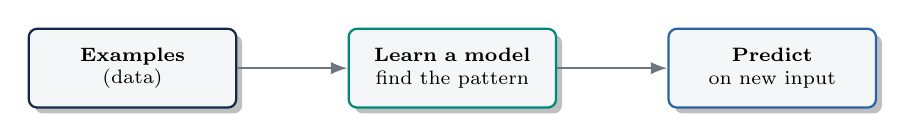
\begin{tikzpicture}[font=\scriptsize,
      b/.style={rectangle, rounded corners=3pt, draw, thick, fill=lightgray, drop shadow,
                align=center, text width=2.4cm, minimum height=1.0cm}]
    \node[b, draw=labnavy] (data) {\textbf{Examples}\\ \scriptsize (data)};
    \node[b, draw=accentteal, right=1.4cm of data] (model) {\textbf{Learn a model}\\ \scriptsize find the pattern};
    \node[b, draw=accentblue, right=1.4cm of model] (pred) {\textbf{Predict}\\ \scriptsize on new input};
    \draw[-{Latex[length=6pt]}, thick, midgray] (data)--(model);
    \draw[-{Latex[length=6pt]}, thick, midgray] (model)--(pred);
  \end{tikzpicture}
  \end{center}
  \vspace{6pt}
  \begin{columns}[t,totalwidth=\textwidth]
    \begin{column}{0.48\textwidth}
      \begin{featbox}{cRAG}{\faTags\ Supervised}
        \scriptsize Learn from \textbf{labeled} examples to predict a label ---
        e.g.\ ``is this passage about grace or law?''
      \end{featbox}
    \end{column}
    \begin{column}{0.04\textwidth}\end{column}
    \begin{column}{0.48\textwidth}
      \begin{featbox}{cEval}{\faObjectGroup\ Unsupervised}
        \scriptsize Find \textbf{structure} without labels --- e.g.\ cluster
        passages by theme, or find the most similar verse.
      \end{featbox}
    \end{column}
  \end{columns}
  \vspace{8pt}
  \begin{center}\small\color{midgray}The machine \emph{finds} the rule from data; we do not write it by hand.\end{center}
\end{frame}

% ---------------------------------------------------------------- deep learning
\begin{frame}{Deep learning: neural networks that learn their own features}
  \begin{columns}[c,totalwidth=\textwidth]
    \begin{column}{0.5\textwidth}
      \begin{center}
      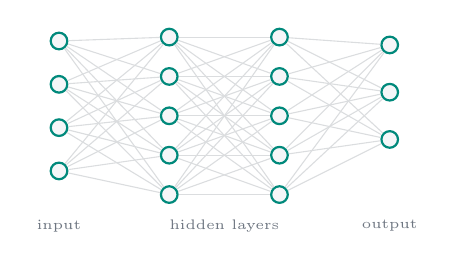
\begin{tikzpicture}[
          n/.style={circle, draw=accentteal, thick, fill=lightgray, minimum size=6pt, inner sep=0pt}]
        \foreach \y in {1,...,4} \node[n] (i\y) at (0,\y*0.55) {};
        \foreach \y in {1,...,5} \node[n] (h\y) at (1.4,\y*0.5-0.25) {};
        \foreach \y in {1,...,5} \node[n] (g\y) at (2.8,\y*0.5-0.25) {};
        \foreach \y in {1,...,3} \node[n] (o\y) at (4.2,\y*0.6+0.35) {};
        \foreach \a in {1,...,4} \foreach \b in {1,...,5} \draw[midgray!25] (i\a)--(h\b);
        \foreach \a in {1,...,5} \foreach \b in {1,...,5} \draw[midgray!25] (h\a)--(g\b);
        \foreach \a in {1,...,5} \foreach \b in {1,...,3} \draw[midgray!25] (g\a)--(o\b);
        \node[font=\tiny,text=midgray] at (0,-0.15) {input};
        \node[font=\tiny,text=midgray] at (2.1,-0.15) {hidden layers};
        \node[font=\tiny,text=midgray] at (4.2,-0.15) {output};
      \end{tikzpicture}
      \end{center}
    \end{column}
    \begin{column}{0.5\textwidth}
      \small
      \begin{itemize}
        \item \textbf{Many layers}, each building a richer representation of the input.
        \item Learns the useful \textbf{features itself} --- no hand-engineering.
        \item Took off with \textbf{big data $+$ GPUs} (2012 onward).
      \end{itemize}
      \vspace{2pt}
      {\scriptsize\color{midgray}Different data, different architecture: CNNs for images, transformers for text.}
    \end{column}
  \end{columns}
  \vspace{4pt}
  \begin{center}\small\color{labnavy}\bfseries Representation learning at scale --- the engine under modern AI.\end{center}
\end{frame}

% ---------------------------------------------------------------- LLMs
\begin{frame}{Large language models: predict the next word, at scale}
  \begin{center}
  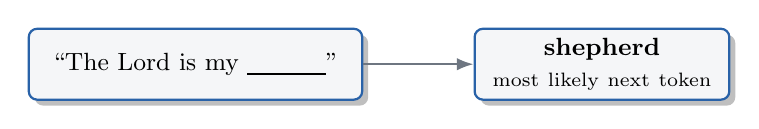
\begin{tikzpicture}[font=\small]
    \node[rectangle, rounded corners=3pt, draw=accentblue, thick, fill=lightgray, drop shadow,
          align=center, text width=4.0cm, minimum height=0.9cm] (ctx)
      {``The Lord is my \underline{\hspace{1.0cm}}''};
    \node[right=1.4cm of ctx, rectangle, rounded corners=3pt, draw=cAgent, thick, fill=lightgray,
          drop shadow, align=center, text width=3.0cm, minimum height=0.9cm] (pred)
      {\textbf{shepherd}\\ \scriptsize most likely next token};
    \draw[-{Latex[length=6pt]}, thick, midgray] (ctx)--(pred);
  \end{tikzpicture}
  \end{center}
  \vspace{2pt}
  \begin{center}\footnotesize\color{midgray}Trained on massive text to predict the next token --- repeated billions of times.\end{center}
  \vspace{6pt}
  \begin{columns}[t,totalwidth=\textwidth]
    \begin{column}{0.48\textwidth}
      \begin{featbox}{accentblue}{\faCheckCircle\ What it gives you}
        \scriptsize Fluent, general language and broad knowledge; it can summarize,
        translate, draft, and reason over text.
      \end{featbox}
    \end{column}
    \begin{column}{0.04\textwidth}\end{column}
    \begin{column}{0.48\textwidth}
      \begin{featbox}{accentgold}{\faExclamationTriangle\ The catch}
        \scriptsize Not a database. It can state a \textbf{false} ``fact'' --- a
        fabricated verse --- with full confidence.
      \end{featbox}
    \end{column}
  \end{columns}
  \vspace{6pt}
  \begin{center}\small\color{labnavy}This is exactly why we add
    \textcolor{cRAG}{\textbf{RAG}} (grounding) and
    \textcolor{cEval}{\textbf{evaluation}}.\end{center}
\end{frame}

% ---------------------------------------------------------------- history of AI (2)
\begin{frame}{Why \emph{now}? Compute + data + a scalable architecture}
  \begin{columns}[c, totalwidth=\textwidth]
    \begin{column}{0.58\textwidth}
      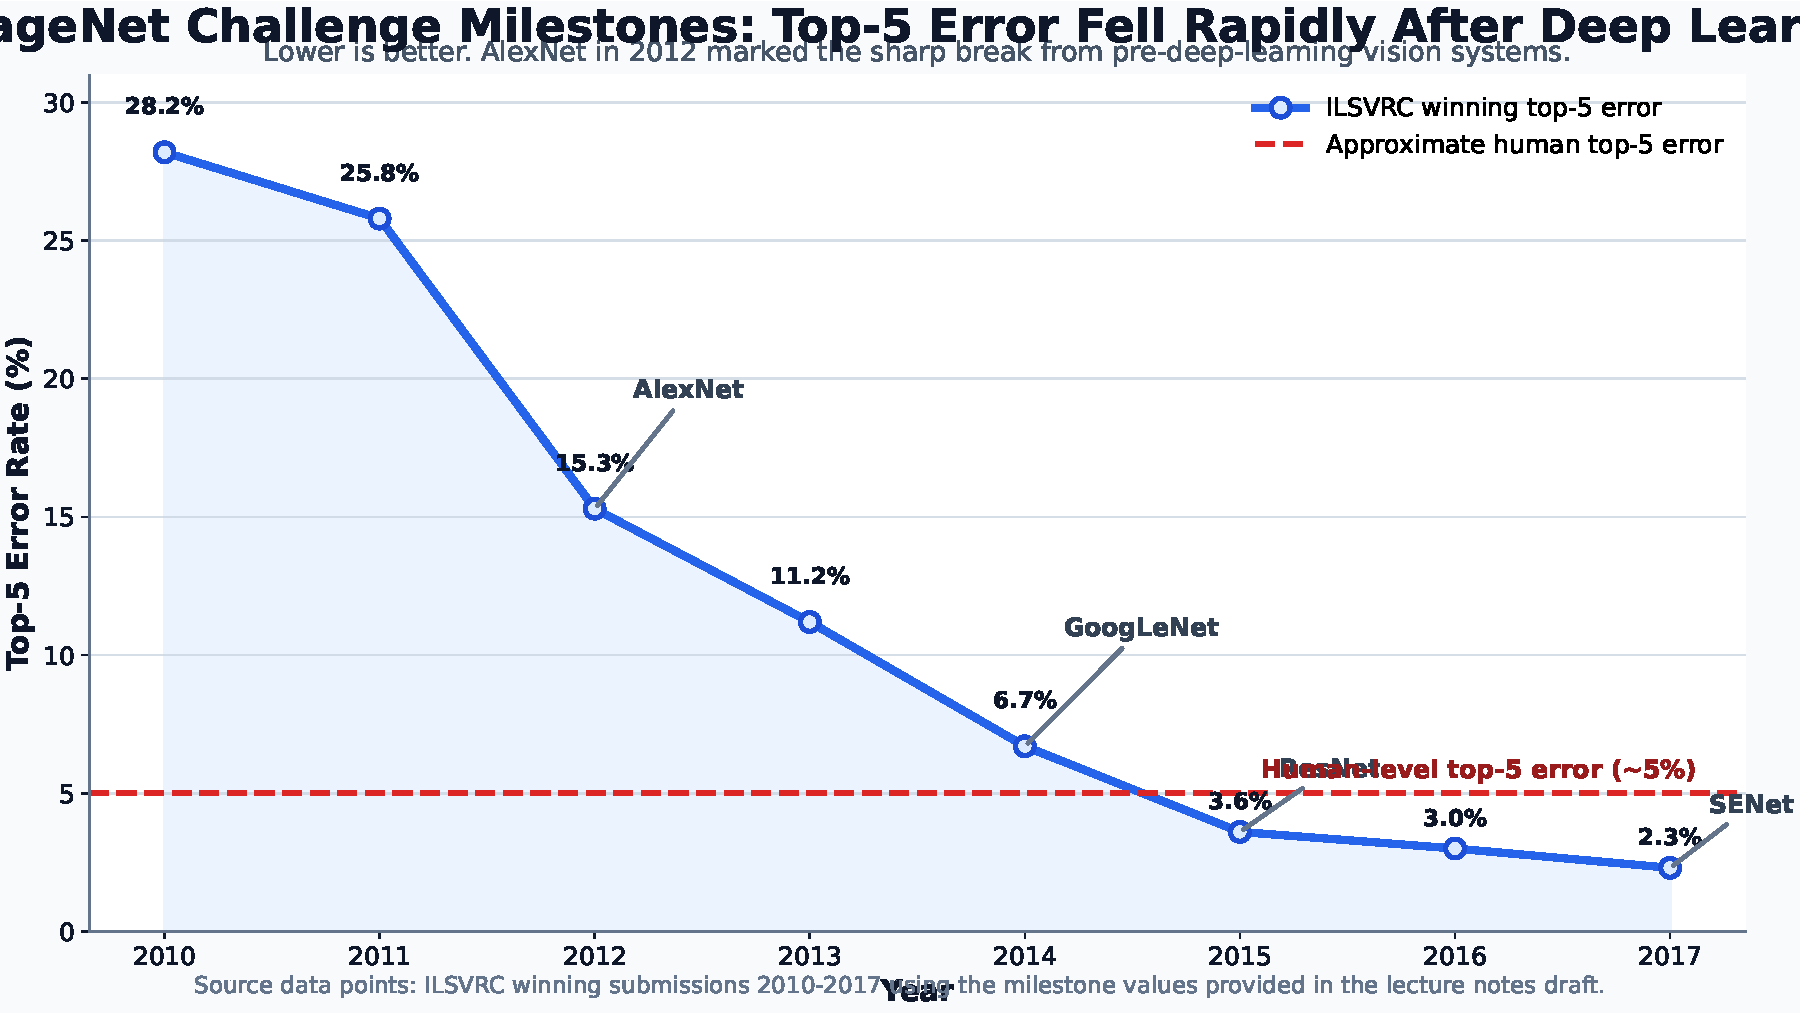
\includegraphics[width=\textwidth,trim=0 12pt 0 36pt,clip]{images/imagenet_accuracy_milestones.pdf}
    \end{column}
    \begin{column}{0.42\textwidth}
      \footnotesize
      \begin{itemize}
        \item \textbf{2012 --- AlexNet.} A deep CNN on GPUs cut ImageNet error
              from ${>}25\%$ to $15.3\%$. Known ideas $+$ GPU compute $+$ big data.
        \item \textbf{2017 --- Transformer.} \emph{Attention Is All You Need}
              replaced recurrence with self-attention $\Rightarrow$ parallel,
              scalable training. The basis for GPT, BERT, Llama, Claude, Gemini.
        \item \textbf{2022 --- ChatGPT.} Made the leap public; the systems story
              is the same --- coordinate compute, memory, and data.
      \end{itemize}
      \vspace{2pt}
      {\color{labnavy}\bfseries This is the wave your project rides.}
    \end{column}
  \end{columns}
\end{frame}

% ---------------------------------------------------------------- LLM vs agent vs system
% Recreated in-deck from ATPESC 2026 agentic_tools_1, slide 4. Source .tex not on disk.
\begin{frame}{LLM, agent, agentic system --- not the same thing}
  \begin{columns}[t, totalwidth=\textwidth]
    \begin{column}{0.48\textwidth}
      \begin{featbox}{labnavy}{\faComments\ LLM}
        \scriptsize
        \begin{itemize}
          \item Primarily \textbf{responds} to a prompt
          \item Generates text, code, or analysis
          \item Usually stops after one answer
          \item Does not manage execution itself
        \end{itemize}
        \vspace{1pt}
        {\scriptsize\color{midgray}Examples: GPT-5, Claude}
      \end{featbox}
    \end{column}
    \begin{column}{0.04\textwidth}\end{column}
    \begin{column}{0.48\textwidth}
      \begin{featbox}{cAgent}{\faRobot\ Agent}
        \scriptsize
        \begin{itemize}
          \item Wraps an LLM with \textbf{tools + memory + control logic}
          \item Can plan, act, observe, and continue
          \item Executes a task instead of only answering
          \item Uses tools and recovers from failures
        \end{itemize}
        \vspace{1pt}
        {\scriptsize\color{midgray}Examples: GPT-5 $\to$ Codex, Claude $\to$ Claude Code}
      \end{featbox}
    \end{column}
  \end{columns}
  \vspace{8pt}
  \begin{calloutbox}[accentteal]
    \small\faSitemap\ \textbf{Agentic system:} the operational stack around one
    or more agents --- tools, memory, permissions, policies, scheduling, user
    interaction, and recovery.
  \end{calloutbox}
\end{frame}

% ---------------------------------------------------------------- LLM to agent
\begin{frame}{What turns an LLM into an \emph{agent}?}
  \begin{center}\small
  An LLM is a \textbf{next-token predictor}: fluent, not a database ---
  and it will confidently \textbf{hallucinate} a verse. Add four things:
  \end{center}
  \vspace{4pt}
  \begin{columns}[t, totalwidth=\textwidth]
    \begin{column}{0.235\textwidth}
      \begin{featbox}{cAgent}{\faTools\ Tools}
        \scriptsize Call a retriever, a calculator, a code runner, the web.
      \end{featbox}
    \end{column}
    \begin{column}{0.02\textwidth}\end{column}
    \begin{column}{0.235\textwidth}
      \begin{featbox}{cRAG}{\faBrain\ Memory}
        \scriptsize Carry state across steps --- what it found, what it decided.
      \end{featbox}
    \end{column}
    \begin{column}{0.02\textwidth}\end{column}
    \begin{column}{0.235\textwidth}
      \begin{featbox}{accentblue}{\faSync\ Plan--act--observe}
        \scriptsize Decompose, act, \emph{look at the result}, decide the next step.
      \end{featbox}
    \end{column}
    \begin{column}{0.02\textwidth}\end{column}
    \begin{column}{0.235\textwidth}
      \begin{featbox}{cEval}{\faCompass\ Autonomy}
        \scriptsize Run many steps toward a goal without a human at each one.
      \end{featbox}
    \end{column}
  \end{columns}
  \vspace{10pt}
  \begin{center}\small\color{labnavy}An LLM answers in one shot. An \textbf{agent} runs the loop.\end{center}
\end{frame}

% ---------------------------------------------------------------- the loop
\begin{frame}{The loop: plan $\to$ act $\to$ observe $\to$ repeat}
  \begin{center}
  \begin{tikzpicture}[font=\small,
      node distance=1.5cm and 1.7cm,
      stg/.style={rectangle, rounded corners=3pt, draw, thick, fill=lightgray,
                  drop shadow, align=center, text width=1.9cm, minimum height=1.0cm}]
    \node[stg, draw=labnavy]  (goal)    {\faBullseye\\ Goal};
    \node[stg, draw=cAgent, right=of goal] (plan) {\faSitemap\\ Plan};
    \node[stg, draw=cRAG, right=of plan]   (act)  {\faTools\\ Act\\ \scriptsize(call a tool)};
    \node[stg, draw=accentblue, right=of act] (obs) {\faEye\\ Observe\\ \scriptsize(read result)};
    \node[stg, draw=cEval, below=of act] (ans) {\faCheckDouble\\ Answer\\ \scriptsize(with citation)};
    \draw[-{Latex[length=6pt]}, thick, midgray] (goal) -- (plan);
    \draw[-{Latex[length=6pt]}, thick, midgray] (plan) -- (act);
    \draw[-{Latex[length=6pt]}, thick, midgray] (act)  -- (obs);
    \draw[-{Latex[length=6pt]}, thick, midgray] (obs.south) to[out=-90,in=0] node[right,font=\scriptsize,text width=1.6cm]{reflect \& loop} (act.east |- ans.east) -- (ans.east);
    \draw[-{Latex[length=6pt]}, thick, cAgent] (obs) to[out=120,in=60] node[above,font=\scriptsize]{not done?} (plan);
  \end{tikzpicture}
  \end{center}
\end{frame}

% ---------------------------------------------------------------- hands-on intro
\begin{frame}{Part 2 --- Hands-on: install the workshop}
  \vspace{4pt}
  \begin{calloutbox}[accentteal]
    \small\faInfoCircle\ \textbf{Claude Code} (Anthropic) and \textbf{Codex}
    (OpenAI) are terminal-based coding agents that live inside your editor ---
    the \emph{agentic AI} we just met, pointed at files. \textbf{You only need one.}
  \end{calloutbox}
  \vspace{8pt}
  \begin{center}
  \begin{tikzpicture}[font=\scriptsize,
      s/.style={rectangle, rounded corners=3pt, draw, thick, fill=lightgray,
                drop shadow, align=center, text width=2.3cm, minimum height=1.15cm}]
    \node[s, draw=accentblue] (vs)   {\faCode\\ \textbf{1. VS Code}\\ + terminal};
    \node[s, draw=cRAG, right=1.3cm of vs] (node) {\faNodeJs\\ \textbf{2. Node.js}\\ (gives npm)};
    \node[s, draw=cAgent, right=1.3cm of node] (agent) {\faRobot\\ \textbf{3. An agent}\\ Claude Code \emph{or} Codex};
    \draw[-{Latex[length=6pt]}, thick, midgray] (vs) -- (node);
    \draw[-{Latex[length=6pt]}, thick, midgray] (node) -- (agent);
  \end{tikzpicture}
  \end{center}
  \vspace{4pt}
  \begin{center}\footnotesize\color{midgray}Use the instructor-provided access. Never paste a personal API key onto a shared machine.\end{center}
\end{frame}

% ---------------------------------------------------------------- install commands
\begin{frame}[fragile]{Install: VS Code $\to$ Node $\to$ one coding agent}
  \begin{columns}[t, totalwidth=\textwidth]
    \begin{column}{0.5\textwidth}
      {\footnotesize\bfseries\color{accentblue}\faCheckCircle\ Prerequisites}
      \begin{enumerate}\footnotesize
        \item Install \textbf{VS Code} --- \texttt{code.visualstudio.com}
        \item Open a terminal: \texttt{Terminal $\to$ New Terminal}
        \item Install \textbf{Node.js (LTS)} --- \texttt{nodejs.org}, then verify:
      \end{enumerate}
      \begin{lstlisting}[style=shell]
node --version
npm  --version
      \end{lstlisting}
    \end{column}
    \begin{column}{0.5\textwidth}
      {\footnotesize\bfseries\color{cAgent}\faRobot\ Pick \emph{one} agent}
      \begin{lstlisting}[style=shell, title=Claude Code (Anthropic)]
npm install -g @anthropic-ai/claude-code
claude
      \end{lstlisting}
      \begin{lstlisting}[style=shell, title=Codex (OpenAI)]
npm install -g @openai/codex
codex
      \end{lstlisting}
      {\scriptsize\color{midgray} First run opens a browser sign-in. Use the
      instructor-provided access.}
    \end{column}
  \end{columns}
\end{frame}

% ---------------------------------------------------------------- feel the loop
\begin{frame}{Feel the loop on purpose --- then you are set for the term}
  \begin{calloutbox}[cAgent]
    \small\faTerminal\ In your agent (\texttt{claude} or \texttt{codex}), type a
    \textbf{two-step} request:\\[4pt]
    \textit{``Make a folder \texttt{notes/}, then inside it create
    \texttt{week1.md} with a bullet list of the three pillars of this course.''}
  \end{calloutbox}
  \vspace{10pt}
  \begin{center}\small
    Watch it \textbf{decompose} the task, \textbf{act}, \textbf{check} the
    result, and \textbf{continue}.\\[3pt]
    {\color{labnavy}\bfseries That is the agentic loop --- the same idea we aim
    at theological corpora in Week 4.}
  \end{center}
\end{frame}

% ---------------------------------------------------------------- wrap
\begin{frame}{Assignment for next week}
  \begin{featbox}{accentblue}{\faUserCircle\ 1. Apply for ALCF access}
    \small
    Apply for an ALCF account at
    \textbf{\texttt{accounts.alcf.anl.gov}}. During the application, request
    to be added to the \textbf{DLIO} project.
  \end{featbox}
  \vspace{7pt}
  \begin{featbox}{accentteal}{\faBookOpen\ 2. Reading assignment}
    \small
    \begin{itemize}
      \item \textbf{Lewis et al.} (2020), \emph{Retrieval-Augmented
        Generation for Knowledge-Intensive NLP Tasks} --- read the abstract
        and introduction.
      \item \textbf{Ji et al.} (2023), \emph{Survey of Hallucination in
        Natural Language Generation} --- read \S1.
      \item \textbf{Write a one-page report} on one of the two papers.
    \end{itemize}
  \end{featbox}
  \vspace{7pt}
  \begin{center}
    {\small\color{midgray}The PDFs are provided with the course materials.}
  \end{center}
\end{frame}

\end{document}
